\documentclass{../notatki}

\usetikzlibrary{chains}

\title{Kryptografia z elementami algebry}

\begin{document}

\tableofcontents

\section{Złożoność obliczeniowa}

\subsection{Dodawanie}

Dodanie dwóch liczb binarnych $a$ i $b$ o długości $n$ ma złożoność $O(n)$,
lub lepiej $O(\log \max(a, b))$.

\subsection{Mnożenie}

Mnożenie dwóch liczb binarnych $a$ i $b$ o długości $n$ ma złożoność $O(n^2)$,
lub lepiej $O(\log^2 \max(a, b))$.

\subsection{Potęgowanie}

Potęgowanie liczby $a$ do potęgi $b$ ma złożoność $O(\log^b a)$.

\subsection{Dzielenie}

Dzielenie liczby $a$ przez $b$ ma złożoność $O(n^2)$.

\subsection{Modulo}

Modulo liczby $a$ przez $b$ ma złożoność $O(n^2)$.

\subsection{Znajdowanie odwrotności}

To zależy od grupy, ale dla $a$ w przypadku $Z_n$ wymaga obliczenia
$n - a$, czyli $O(\log \max(a, n))$. W przypadku $Z_n^\times$ wymaga użycia
rozszerzonego algorytmu Euklidesa. Ten wykonuje w najgorszym przypadku
$a$ iteracji, więc złożoność wynosi $O(a \log^2 \max(a, n))$.

\section{Szyfr Shannona}

Szyfr według Shannon'a jest zdefiniowany jako:
$$
\pi = (E, D) : (C, M, K)
$$
gdzie schemat szyfrujący $E$ i schemat deszyfrowania $D$ są funkcjami:
$$
E: M \times K \rightarrow C
$$
$$
D: C \times K \rightarrow M
$$

$$
D(k, E(k, m)) = m
$$

\subsection{Szyfr XOR}

$$
K = M = C = \{0, 1\}^L
$$

$$
E(m, k) = m \oplus k
$$
$$
D(c, k) = c \oplus k
$$

\subsection{Bezpieczeństwo doskonałe}

Niech $\pi$ będzie szyfrem Shannona. Rozważmy eksperyment losowy, w którym
zmienna losowa $K$ ma rozkład jednostajny nad $K$. Jeśli zachodzi:
$$
\forall_{m_0, m_1 \in M} \forall_{c \in C} P(E(k, m_0) = c) = P(E(k, m_1) = c)
$$
to mówimy, że szyfr $\pi$ jest szyfrem doskonałym.

Jeśli $\pi$ jest szyfrem doskonałym, to $|K| \ge |M|$.

\section{Struktury algebraiczne}

\begin{enumerate}
  \item $\forall_{a, b \in G} a * (b * c) = (a * b) * c$
  \item $\forall_{a, b \in G} a * b = b * a$
  \item $\exists_{e \in G} \forall_{a \in G} a * e = a$
  \item $\forall_{a \in G} a^{-1} = e$
\end{enumerate}

\begin{itemize}
  \item półgrupa: 1
  \item monoid: 1, 3
  \item grupa: 1, 3, 4
  \item grupa abelowa: 1, 2, 3, 4
\end{itemize}

Zawsze istnieje tylko jeden element neutralny operacji.
Rzędem grupy jest moc zbioru $G$.

$$\varphi(n) = |\{a \in \mathbb{Z}_n : \gcd(a, n) = 1\}|$$

\subsection{Podgrupa}

Niech $H$ będzie podgrupą grupy $G$. Wtedy:
$$
\forall_{a, b \in H} a * b \in H
$$
$$
\forall_{a \in H} a^{-1} \in H
$$
Na przykład, dla $\mathbb{Z}_{10} = \{0, 1, 2, 3, 4, 5, 6, 7, 8, 9\}$,
$H = \{0, 2, 4, 6, 8\}$ jest podgrupą grupy $\mathbb{Z}_{10}$.

\subsection{Generatory}

$$
\langle g \rangle = \{g^k : k \in \mathbb{Z}\}
$$

Grupa cykliczna, to grupa, która posiada co najmniej jednoelementowy zbiór
generatorów. $\exists_{g \in G} \langle g \rangle = G$

\subsection{Warstwy}

Dla podgrupy $H$ grupy $G$, warstwą lewostronną $H$ wyznaczoną przez
$a \in G$ jest zbiór:
$$
\begin{cases}
  a + H = \{a + h : h \in H\}\\
  aH = \{ah : h \in H\}
\end{cases}
$$

Warstwy są identyczne, albo rozłączne. Warstwy $aH$ i $bH$ są sobie
równe kiedy $a^{-1}b \in H$. Suma mnogościowa
warstw jest równa grupie $G$. Indeksem podgrupy $H$ w grupie $G$ ($G
: H$) nazywamy moc zbioru warstw względem podgrupy $H$.
$$
G : H = \frac{|G|}{|H|}
$$
Rząd podgrupy $H$ jest dzielnikiem rzędu grupy $G$.

\subsection{Homomorfizmy}

$f: G \to G'$
nazywamy homomorfizmem grupy $G$ w grupę $G'$, jeśli zachodzi:
$$
f(a + b) = f(a) + f(b)
$$
$$
f(ab) = f(a)f(b)
$$

Jeśli:
\begin{itemize}
  \item $f$ jest iniekcją, to mówimy że $f$ jest monomorfizmem.
  \item $f$ jest suriekcją, to mówimy że $f$ jest epimorfizmem.
  \item $f$ jest bijekcją, to mówimy że $f$ jest izomorfizmem.
\end{itemize}

Z własności homomorfizmu wynika, że $f(e) = f(ee) = f(e)f(e) = e'$
oraz $f(a^{-1}) = f(a)^{-1}$ i $f(a)f(a^{-1}) = f(e)$.

Zbiór $Ker(f) = \{a \in G : f(a) = e'\}$ nazywamy jądrem homomorfizmu $f$.

Zbiór $Im(f) = \{f(a) : a \in G\}$ nazywamy obrazem homomorfizmu $f$.

\section{Problemy}

\subsection{Problem logarytmu dyskretnego (DL)}

Niech $G = \langle g \rangle$. Problemem jest znalezienie $x$
takiego, że $g^x = a$. W zależności od grupy oraz jej rozmiaru,
ten problem może być niezwykle trudny.

\begin{figure}[h]
  \centering
  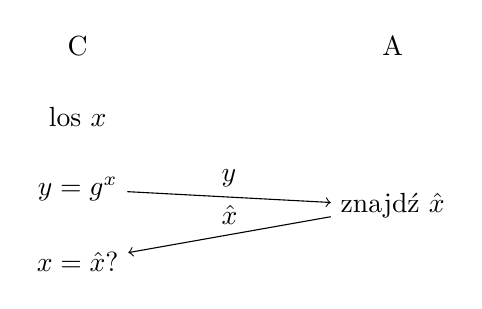
\begin{tikzpicture}[node distance=4mm]
    \node (C) at (0,0) {C};
    \node (A) at (4,0) {A};

    \begin{scope}[start chain=going below]
      \node[on chain, below=of C] (c1) {los $x$};
      \node[on chain] (c2) {$y=g^x$};
      \node[on chain] (c3) {$x=\hat{x}$?};
    \end{scope}

    \node[below=1.5cm of A] (a1) {znajdź $\hat{x}$};

    \draw[->] (c2)  -- node[midway, above] {$y$} (a1);
    \draw[->] (a1)  -- node[midway, above] {$\hat{x}$} (c3);
  \end{tikzpicture}
  \caption{Formalizm gry dla problemu logarytmu dyskretnego}
\end{figure}

\subsection{Problem DDH}

Mamy daną grupę cykliczną $G = \langle g \rangle$, rzędu
$q$, gdzie $q$ jest liczbą pierwszą. Losujemy $\alpha, \beta, \gamma
\in \mathbb{Z}_q$. Następnie obliczamy:
$$
u = g^\alpha, v = g^\beta, w_0 = g^{\alpha \beta}, w_1 = g^\gamma
$$
Celem problemu, jest odgadnięcie $b$, dla danego $u, v, w_b$.

\begin{figure}[h]
  \centering
  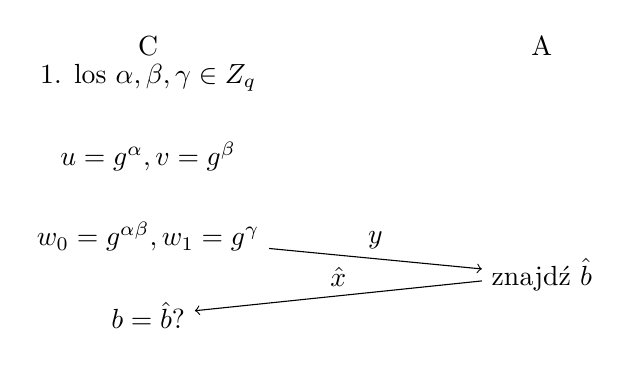
\begin{tikzpicture}[node distance=4mm]
    \node (C) at (0,0) {C};
    \node (A) at (5,0) {A};

    \begin{scope}[start chain=going below]
      \node[on chain, below of=C] (c1) {1. los $\alpha,
        \beta, \gamma \in
      \mathbb{Z}_q$};
      \node[on chain] (c2) {$u = g^\alpha, v = g^\beta$};
      \node[on chain] (c3) {$w_0 = g^{\alpha \beta}, w_1 = g^{\gamma}$};
      \node[below of=A, yshift=-2.5cm] (textA) {znajdź $\hat{b}$};
      \node[on chain] (c4) {$b = \hat{b}$?};
    \end{scope}

    \draw[->] (c3)  -- node[midway, above] {$y$} (textA);
    \draw[->] (textA)  -- node[midway, above] {$\hat{x}$} (c4);
  \end{tikzpicture}
  \caption{Formalizm gry dla problemu DDH}
\end{figure}

\subsection{CDH}

Mamy daną grupę cykliczną $G = \langle g \rangle$, rzędu
$q$, gdzie $q$ jest liczbą pierwszą. Losujemy $\alpha, \beta, \gamma
\in \mathbb{Z}_q$. Następnie obliczamy:
$$
u = g^\alpha, v = g^\beta, w = g^{\alpha \beta}
$$
Celem problemu, jest odgadnięcie $w$, dla danego $u, v$.

\begin{figure}[h]
  \centering
  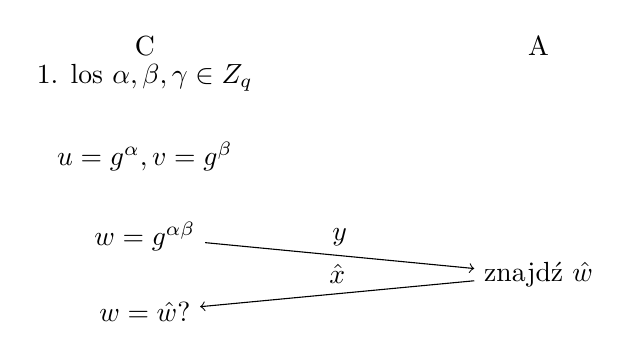
\begin{tikzpicture}[node distance=4mm]
    \node (C) at (0,0) {C};
    \node (A) at (5,0) {A};

    \begin{scope}[start chain=going below]
      \node[on chain, below of=C] (c1) {1. los $\alpha,
        \beta, \gamma \in
      \mathbb{Z}_q$};
      \node[on chain] (c2) {$u = g^\alpha, v = g^\beta$};
      \node[on chain] (c3) {$w = g^{\alpha \beta}$};
      \node[below of=A, yshift=-2.5cm] (textA) {znajdź $\hat{w}$};
      \node[on chain] (c4) {$w = \hat{w}$?};
    \end{scope}

    \draw[->] (c3)  -- node[midway, above] {$y$} (textA);
    \draw[->] (textA)  -- node[midway, above] {$\hat{x}$} (c4);
  \end{tikzpicture}
  \caption{Formalizm gry dla problemu CDH}
\end{figure}

\section{Schematy}

\subsection{Protokół DH}

Mamy daną grupę cykliczną $G = \langle g \rangle$, rzędu
$q$, gdzie $q$ jest liczbą pierwszą.
Protokół Diffie-Hellman (DH), polega na losowym wybraniu sekretów przez dwóch
użytkowników (A, B) $\alpha, \beta \in \mathbb{Z}_q$. Obliczeniu szyfrogramów
$u = g^\alpha, v = g^\beta$, a następnym wysłaniu $u$ i $v$. Sekret wspólny
$s = g^{\alpha \beta}$.

\begin{figure}[h]
  \centering
  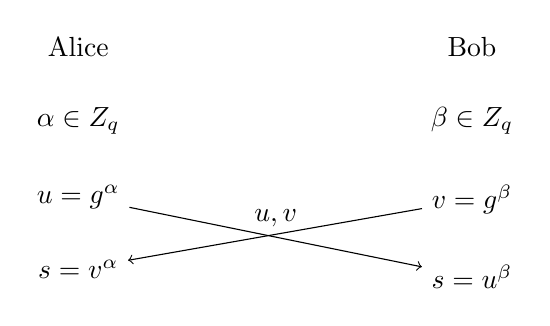
\begin{tikzpicture}[node distance=4mm]
    \node (C) at (0,0) {Alice};
    \node (A) at (5,0) {Bob};

    \begin{scope}[start chain=going below]
      \node[on chain, below=of C] (alpha) {$\alpha \in \mathbb{Z}_q$};
      \node[on chain] (u)     {$u = g^\alpha$};
      \node[on chain] (s1)     {$s = v^{\alpha}$};
    \end{scope}

    \begin{scope}[start chain=going below]
      \node[on chain, below=of A] (beta) {$\beta \in \mathbb{Z}_q$};
      \node[on chain] (v)      {$v = g^\beta$};
      \node[on chain] (s2)      {$s = u^\beta$};
    \end{scope}

    \draw[->] (u) -- node[midway, above] {$u, v$} (s2);
    \draw[->] (v) -- (s1);
  \end{tikzpicture}
  \caption{Formalizm gry dla protokołu DH}
\end{figure}

Protokół jest odporny na atak pasywny (tylko czytanie). Z kolei, jest podatny
na atak jeśli atakujący ma wpływ na kanał komunikacji, chociażby poprzez atak
Man-in-the-middle.

\subsection{Schemat szyfrowania z kluczem publicznym}

$$
\varepsilon = (G, E, D) \text{ nad } (M, C, K)
$$
gdzie $G: \mathbb{N} \to K$, $E: K \times M \to C$, $D: K \times C \to M$.

$$
(pk, sk) = G(\lambda)
$$
$$
C = E(pk, m)
$$
$$
M = D(sk, C)
$$

\section{Ataki}

\subsection{Man-in-the-middle}

Jeśli atakujący ma wplyw na kanał komunikacji, to może przechwycić komunikaty
podczas przekazywania kluczy. W takim momencie, może się podszyć pod drugą
stronę, aby uzyskać dostęp do klucza prywatnego. Równocześnie może
przekazywać dalej komunikację, aby ukryć swoją obecność. W ten sposób
zna obydwa sekrety i tylko siedzi po środku.

\subsection{Bezpieczeństwo semantyczne}

Dla pewnego $\varepsilon = (G, E, D)$, atakujący ma dostęp do klucza
publicznego $pk$. Wybiera on dwie wiadomości $m_0, m_1 \in M$. Przeciwnik
wybiera jedną wiadomość $b \in \{0, 1\}$, szyfruje ją $c = E(pk, m_b)$ i zwraca
atakującemu. Atakujący musi zgadnąć $b$.

\begin{figure}[h]
  \centering
  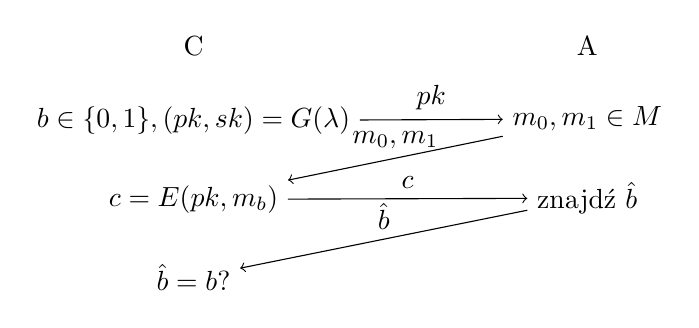
\begin{tikzpicture}[node distance=4mm]
    \node (C) at (0,0) {C};
    \node (A) at (5,0) {A};

    \begin{scope}[start chain=going below]
      \node[on chain, below=of C] (c1) {$b \in \{0, 1\}, (pk, sk) =
      G(\lambda)$};
      \node[on chain] (c2)     {$c = E(pk, m_b)$};
      \node[on chain] (c3)     {$\hat{b} = b$?};
    \end{scope}

    \begin{scope}[start chain=going below]
      \node[on chain, below=of A] (a1) {$m_0, m_1 \in M$};
      \node[on chain] (a2)      {znajdź $\hat{b}$};
    \end{scope}

    \draw[->] (c1) -- node[midway, above] {$pk$} (a1);
    \draw[->] (a1) -- node[midway, above] {$m_0, m_1$} (c2);
    \draw[->] (c2) -- node[midway, above] {$c$} (a2);
    \draw[->] (a2) -- node[midway, above] {$\hat{b}$} (c3);
  \end{tikzpicture}
  \caption{Formalizm gry dla bezpieczeństwa semantycznego}
\end{figure}

\subsection{Atak CDA}

Jest to powielona wersja bezpieczeństwa semantycznego. Wielokrotnie atakujący
może tworzyć wiadomości i dostawać losowy kryptogram na podstawie ich. To czyni
ten atak o wiele trudniejszym niż bezpieczeństwo semantyczne.

\section{RSA}

Asymetryczny algorytm szyfrujący, w którym każda strona ma parę
kluczy: publiczny i prywatny. Enkrypcja odbywa się przy pomocy klucza
publicznego drugiej strony, a dekrypcja przy pomocy klucza prywatnego.

\subsection{Definicja}

Dla danych liczb pierwszych $p$ i $q$.

$$
n = pq
$$
$$
\varphi(n) = (p-1)(q-1)
$$
Następnie wybieramy liczbę $e$ względnie pierwszą z $\varphi(n)$.
Klucz prywatny $d$ musi spełniać warunek $ed \equiv 1
\pmod{\varphi(n)}$, zatem
$$
d = e^{-1} \pmod{\varphi(n)}
$$
$(n, e)$ tworzy klucz publiczny, a $(n, d)$ klucz prywatny.

Szyfrowanie wiadomości $M$ odbywa się za pomocą wzoru:
$$
C = M^e \pmod{n}
$$
Odkrycie wiadomości $M$ odbywa się za pomocą wzoru:
$$
M = C^d \pmod{n}
$$

\subsection{Trudność problemu}

Trudność wynika ze znalezienia $\varphi(n)$, a ponieważ weryfikacja
czy znalezione $\varphi(n)$ jest poprawne wymaga zastosowania rozszerzonego
algorytmu Euklidesa; odszyfrowanie wiadomości $C$ wymaga znalezienia $d$.

\subsection{Przykład}

$$
p = 7, q = 11 \Rightarrow n = 77, \varphi(n) = 60
$$
$$
e = 13 \Rightarrow d = 37 \Rightarrow
\begin{cases}
  (n, e) = (77, 13) \\
  (n, d) = (77, 37)
\end{cases}
$$

$$
M = 15 \Rightarrow C = 15^{13} \pmod{77} = 64
$$
$$
C = 64 \Rightarrow M = 64^{37} \pmod{77} = 15
$$

\end{document}
